%%%%%%%%%%%%%%%%%%%%%%%%%%%%%%%%%%%%%%%%%%%%%%%%%%%%%%%%%%%%%%%%%%%%%%%%%%%%%%%%%%
\begin{frame}[fragile]\frametitle{}
\begin{center}
{\Large Yama यम}
\end{center}
\end{frame}

%%%%%%%%%%%%%%%%%%%%%%%%%%%%%%%%%%%%%%%%%%%%%%%%%%%%%%%%%%%
\begin{frame}[fragile]\frametitle{Introduction}


	\begin{itemize}
	\item Restraints, or things to avoid.
	\item Like commandments.
	\end{itemize}

\end{frame}


%%%%%%%%%%%%%%%%%%%%%%%%%%%%%%%%%%%%%%%%%%%%%%%%%%%%%%%%%%%
\begin{frame}[fragile]\frametitle{Introduction}

Ahimsa Satyasteya Bhtahmacharya-parigraha Yamah

अहिंसा-सात्यास्तेय-ब्रह्मचर्यापरिग्रहा यम:||

	\begin{itemize}
	\item Yama  is 
the  first  discipline  in  attaining 
perfection.
	\item Non-violence,  truthfulness, abstaining  from  appropriating things  belongings  to  other, 
purity  in  thoughts,  words  \& 
deed.  And  non-acquisition  of 
things  are  the  essential, 
components of Yama. 

	\end{itemize}

{\tiny (Ref : Patanjali's Yoga Sutra: How to Live by the Yama - Judith Lasater)}

\end{frame}


%%%%%%%%%%%%%%%%%%%%%%%%%%%%%%%%%%%%%%%%%%%%%%%%%%%%%%%%%%%
\begin{frame}[fragile]\frametitle{Ethical Foundations}

	\begin{itemize}
	\item Ahimsa (अहिंसा): non-violence
	\item Satya (सत्य): benevolent truth,absence of falsehood
	\item Asteya (अस्तेय): non-stealing
	\item Brahmacharya (ब्रह्मचर्य): spiritual advancement by education and training. Some traditions associate Brahmacharya with celibacy.
	\item Aparigraha (अपरिग्रह): non-appropriation,absence of avarice.

	\end{itemize}

\end{frame}


%%%%%%%%%%%%%%%%%%%%%%%%%%%%%%%%%%%%%%%%%%%%%%%%%%%%%%%%%%%
\begin{frame}[fragile]\frametitle{Ahimsa (अहिंसा) Non-violence}

   \begin{columns}
    \begin{column}[t]{0.7\linewidth}
	
	\begin{itemize}
	\item Not killing
	\item Not having violent thoughts
	\item Not having violent intentions
	\item Having a considerate attitude; not harming others
	\item Kindness; friendliness
	\item Thoughtful consideration of other people and things
	\item Love
	\item Effects of Ahimsa: eliminating violence around you
	\end{itemize}
	
    \end{column}
    \begin{column}[t]{0.3\linewidth}	
\begin{center}
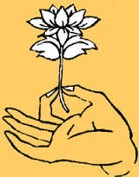
\includegraphics[width=0.8\linewidth,keepaspectratio]{yog24}

\end{center}


    \end{column}
  \end{columns}
  
  \tiny{(Ref: Yoga: The art of happiness - Yoga Integral Esoterique)}

\end{frame}

%%%%%%%%%%%%%%%%%%%%%%%%%%%%%%%%%%%%%%%%%%%%%%%%%%%%%%%%%%%
\begin{frame}[fragile]\frametitle{Satya (सत्य) The truth}
   \begin{columns}
    \begin{column}[t]{0.7\linewidth}
	
	\begin{itemize}
	\item Not speaking the truth can misguide others and ourselves in the end
	\item If speaking the truth has negative consequences for another, then it is better to say nothing (not breaking ahimsa - non-violence)
	\item The truth can be relative in our world of opposite poles or duality (there is always a bigger or another truth that takes the place of the previous one).
	\item  Essentially the truth is one with our inner Consciousness – called Atman or Superior Self.
	\item वाकसिद्धि Vaksiddhi:  the power to materialize what we are saying.

	\end{itemize}
    \end{column}
    \begin{column}[t]{0.3\linewidth}		
\begin{center}

\includegraphics[width=0.8\linewidth,keepaspectratio]{yog25}

\end{center}

    \end{column}
  \end{columns}
  
  \tiny{(Ref: Yoga: The art of happiness - Yoga Integral Esoterique)}

\end{frame}

%%%%%%%%%%%%%%%%%%%%%%%%%%%%%%%%%%%%%%%%%%%%%%%%%%%%%%%%%%%
\begin{frame}[fragile]\frametitle{Asteya (अस्तेय) Non-stealing}
   \begin{columns}
    \begin{column}[t]{0.7\linewidth}
	
	\begin{itemize}
	\item Taking nothing that does not belong to us
	\item Not taking what belongs to another without permission, and not using something for a different purpose to that intended, or beyond the time permitted by its owner
	\item If we  ask for others' time when it is not freely given, it is, in effect, stealing.
	\item Also renouncing desires
	\item Effects: development of clairvoyance or intuition, discovering precious  treasures  around yourself

	\end{itemize}
    \end{column}
    \begin{column}[t]{0.3\linewidth}	
\begin{center}

\includegraphics[width=0.8\linewidth,keepaspectratio]{yog26}

\end{center}
    \end{column}
  \end{columns}
  
  \tiny{(Ref: Yoga: The art of happiness - Yoga Integral Esoterique)}

\end{frame}

%%%%%%%%%%%%%%%%%%%%%%%%%%%%%%%%%%%%%%%%%%%%%%%%%%%%%%%%%%%
\begin{frame}[fragile]\frametitle{Brahmacharya (ब्रह्मचर्य) Control of sexual function  }
   \begin{columns}
    \begin{column}[t]{0.7\linewidth}
	
	\begin{itemize}
	\item Brahmacharya: retention, stopping, abstinence 
	\item Literally means wise use of sexual energy (brah-muh-char-yuh) 
	\item Controlling or preserving  sexual energy (not ejaculating or preserving feminine sexual fluids) allows control of all other types of energies because sexual energy is the most powerful of all energies (it can create life)
	\item Wise use: transforming our sexual energy into love, mental or spiritual energy (by transmutation and sublimation)
	\item Abstinence - not having sexual relations (except involuntary ejaculation) 


	\end{itemize}
	    \end{column}
    \begin{column}[t]{0.3\linewidth}
\begin{center}
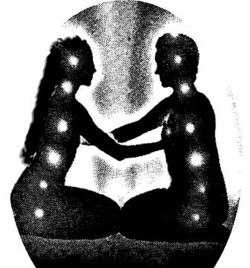
\includegraphics[width=0.8\linewidth,keepaspectratio]{yog27}

\end{center}
    \end{column}
  \end{columns}
  
  \tiny{(Ref: Yoga: The art of happiness - Yoga Integral Esoterique)}

\end{frame}

%%%%%%%%%%%%%%%%%%%%%%%%%%%%%%%%%%%%%%%%%%%%%%%%%%%%%%%%%%%
\begin{frame}[fragile]\frametitle{Aparigraha (अपरिग्रह) Non-accumulation }
   \begin{columns}
    \begin{column}[t]{0.7\linewidth}
	
	\begin{itemize}
	\item Taking only what is necessary, and not taking advantage of a situation or acting greedily
	\item Taking only what we have earned
	\item Many possessions lead to many worries, and energy spent to maintain the accumulated objects
	\item If we need more, the Universe will provide for us.
	\item Effects: acquiring the ability to see previous lives.  When everything is lost, what stays is the immortal Spirit, or Atman, which passes from one life to another, to another
	\end{itemize}
	    \end{column}
    \begin{column}[t]{0.3\linewidth}
\begin{center}

\includegraphics[width=0.8\linewidth,keepaspectratio]{yog28}

\end{center}
    \end{column}
  \end{columns}
  
  \tiny{(Ref: Yoga: The art of happiness - Yoga Integral Esoterique)}

\end{frame}

%%%%%%%%%%%%%%%%%%%%%%%%%%%%%%%%%%%%%%%%%%%%%%%%%%%%%%%%%%%
\begin{frame}[fragile]\frametitle{Summary}

\begin{center}
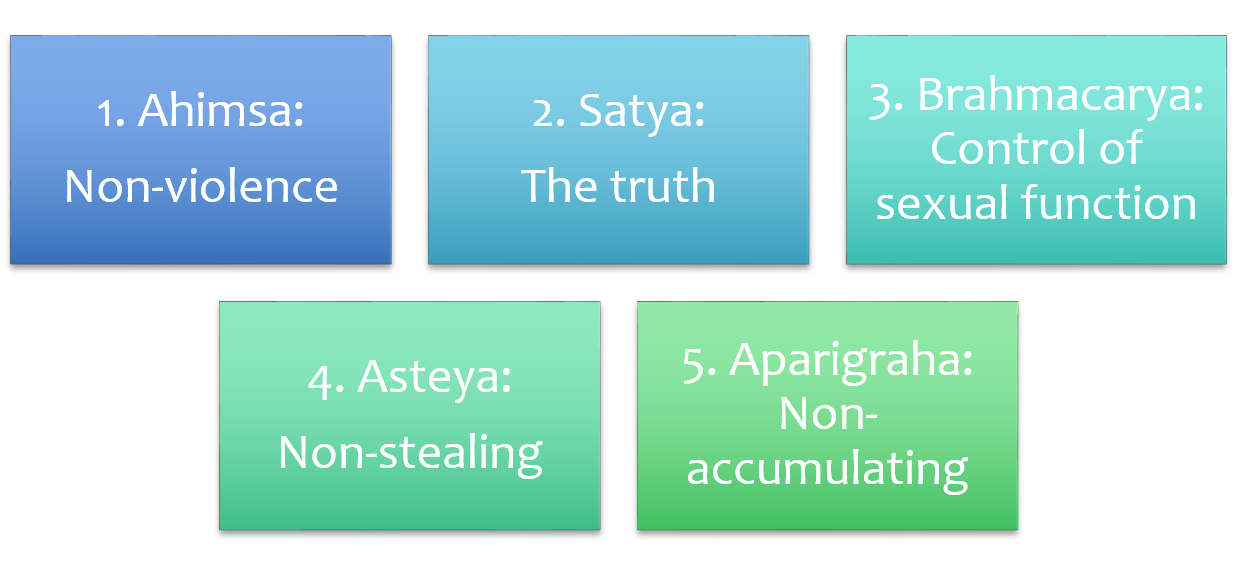
\includegraphics[width=0.8\linewidth,keepaspectratio]{yog29}

\end{center}

  
  \tiny{(Ref: Yoga: The art of happiness - Yoga Integral Esoterique)}

\end{frame}